\subsubsection{Admin}
  The final type of user in CPP: Connect is the department administrator, for this example we will describe a journey our supervisor and the current CPP administrator himself, William Knottenbelt, might take through the system.
  \paragraph{Sign up:}
    Since the software is primarily for the Department of Computing, with other departments being given access at a later date, we have kept initial department creation to be asked for to the database manager. 
    Therefore our system in it's earliest stages will be handed over to the Department of Computing with William Knottenbelt as the initial administrator.

  \paragraph{Dashboard:}
    On signing in Will is directed to his dashboard, where he can then easily add other department administrators, such as Sernea Coultress, the Department of Computing's Industrial Liaison Officer in order to balance the work load on the site. This is very much like a company administrator's new administrator process.

    % TODO: DASH PICTURE ONCE ALL STUFF IS IN HAVE SOME REJECTION/APPROVALS PENDING
    % TODO MAKE SURE AMAZON EMAILS AND PALANTIR ACCEPT

    Will also has the option to set company notifications which will be shown whenever a company tries to create a new event or placement. For example he can add URLs to health and safety placement forms etc. that must be filled out in order for industrial placements to be approved by the college. 

    Will then notices his approvals section, here he must approve any mass student emails a company has sent. Will can also view the direct email list in order to take note of who companies have contacted individually, in this case Jack.
    %TODO PRINT SCREEN DIRECT EMAILS?

    %TOOD: Don't have XXX pick a company for print screens
    He also can approve new companies permissions to access his department's students or just to advertise events and placements. Here he deems Palantir acceptable since they too are a Corporate Partner.

  \paragraph{Students:}
    By clicking `Students' in the navigation bar, Will is able to manage all students for his department.
    Whilst here Will remembers that he has been asked by a current student, Sarah, to sign her up. Although she should be expected to sign herself up to reduce the work load for Will, he decides this once just to allow it.
    He then clicks on the `New Student' button which allows him to register Sarah's user details and is then taken to a page where he can add more information if necessary, or leave it to allow Sarah to do it herself.
    \begin{figure}[H]\centering
    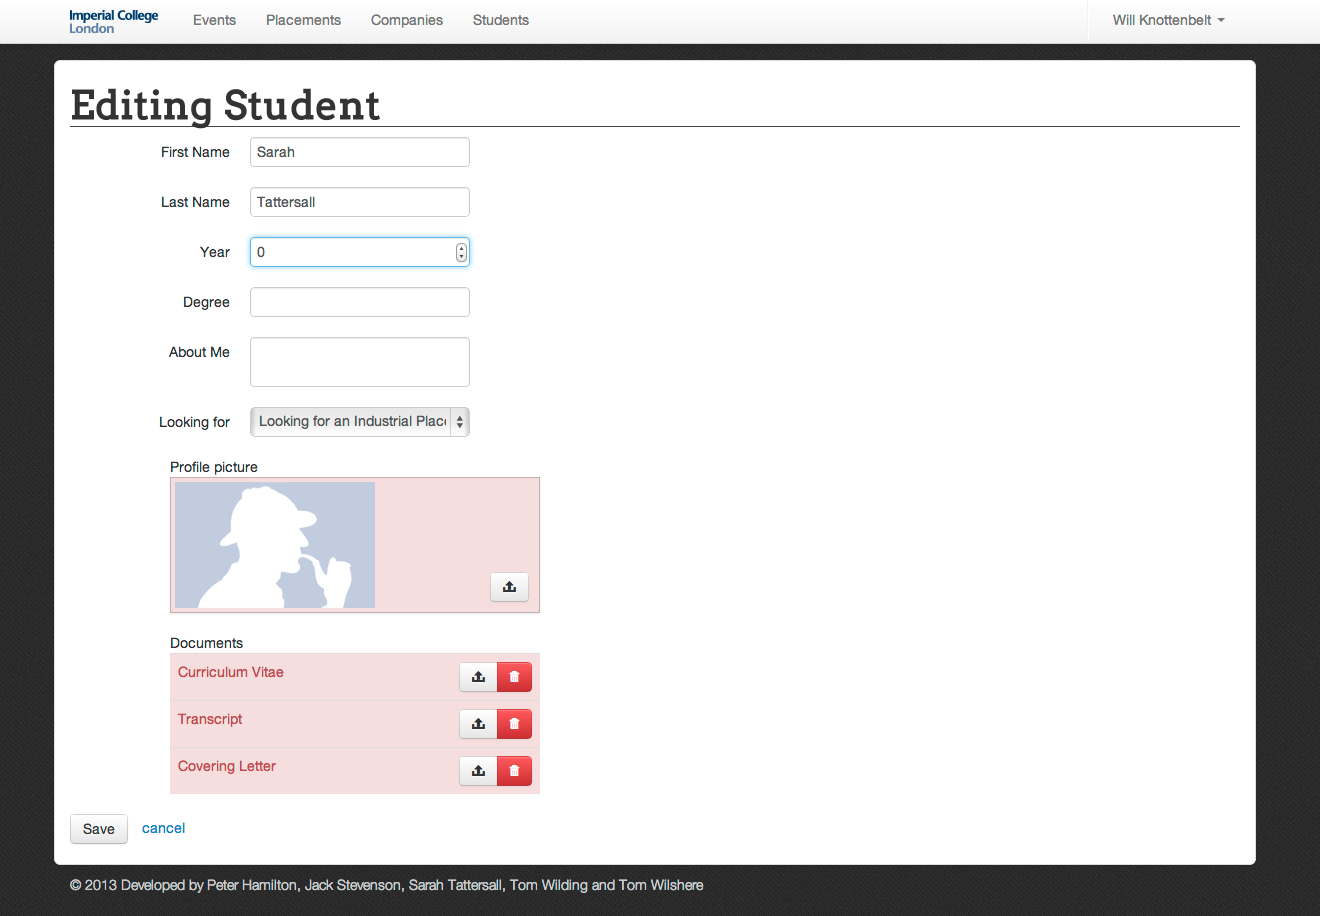
\includegraphics[scale=0.3]{images/user_experiences/admin/admin_student_edit}
    \caption{Student edit page for department administrators}
    \end{figure}

    Will also has the right to be able to delete any students who have either left the department or are causing a problem on the site. We hope the latter will not happen but it is a risk that could arise when students are allowed to develop their own profile.

  \paragraph{Companies:}
    Will can edit, create, and delete companies in exactly the same way as students and can also be directed to a page the edits the companies contacts directly.

    \begin{figure}[H]\centering
    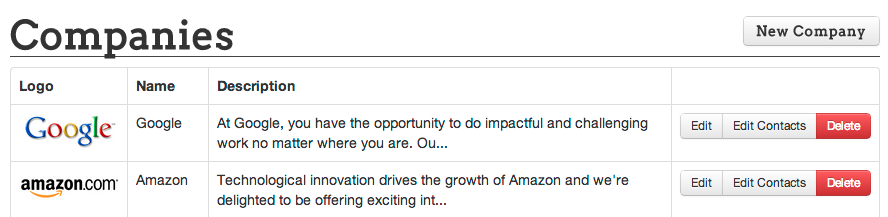
\includegraphics[scale=0.5]{images/user_experiences/admin/admin_company_edit_options}
    \caption{Department administrator company edit options}
    \end{figure}

  \paragraph{Emails:}
    Much like companies, Will may wish to send an email out to the department's students. Instead of using the Imperial email system, he chooses to send it on CPP: Connect because the tagging system allows smart elimination of students who do not want to receive these sort of emails (thus reducing the number of complaints he receives!). Will chooses to send an email out detailing some interesting competitions which students can get involved in. Since he's a department administrator he does not have to receive approval for these and they are sent straight away.
